% !TeX root = ./document.tex
\documentclass[document]{subfiles}
\begin{document}
\chapter{Сопряжённые пространства}
\section{Сопряженное пространство к $L^p$}

На самом деле, в этой части всё докажем только для $l$, для $L$ только простую часть.

Напоминание о том, что мы думаем о мерах: $(X, U, \mu)$ --- пространство с мерой, $\mu$ --- $\sigma$-конечная, то есть $X = \bigcup^\infty_{j=1} X_j, \mu(X_j) < +\infty$.
$\mu$ --- полная мера, то есть если $A \subset U, \mu A = 0$, то  $\forall B \subset A \Rightarrow B \in U, \mu(B) = 0$

\begin{theorem}[сопряженное к $L^p(X, U, \mu)$]
    2 случая, во втором очень важно, что бесконечность не включается!
    \begin{enumerate}
        \item $1 \leq p \leq +\infty$
         \begin{gather*}
            g \in L^q(X,\mu) \quad \frac{1}{p} + \frac{1}{q} = 1 \\
            g \text{ --- фиксирована}, h \in L^p, F_g(h) \coloneqq \int_X h(x) g(x) d\mu \Rightarrow F_g \in (L^p)^* \\
            \norm{F_g} = \norm{g}_{L^q}
        \end{gather*}
        \item $1 \leq p < +\infty$, $F \in (L^p)^* \Rightarrow \: \exists! g \in L^q \text{ т.ч. } F = F_g$
    \end{enumerate}
\end{theorem}

\begin{proof}[1 утверждение]
    Ну тут совсем легко. $F_g \in \Lin(L^p, \bC)$ --- очевидно, просто потому что интеграл --- линейное действие. Теперь, как его оценить?
    \begin{gather*}
        g \in L^q, h \in L^p, \abs{F_g(h)} = \abs{\int_X hg d\mu} \leq \left[\left[\text{ Гельдер }\right]\right] \norm{h}_p \norm{g}_q \: \forall h \in L^p
        \intertext{мы уже отмечали, что неравенство верно даже для бесконечных $p$ и $q$}
        \Rightarrow F_g \in (L^p)^*, \norm{Fg} \leq \norm{g}_q
        \intertext{чтобы получить неравенство в другую сторону, предъявим так называемую пробную функцию, на которой будет выполняться неравенство. Пусть сначала 
        $1 < p \leq +\infty \Rightarrow 1 \leq q < +\infty$}
        U(x) \coloneqq \begin{cases}
             \frac{\overline{g(x)}}{\abs{g(x)}} \abs{g(x)}^{q-1} & g(x) \ne 0 \\
             0 & g(x) = 0
        \end{cases}, \overline{g(x)} \text{ --- комплексное сопряжение}
        \intertext{Проверим, что $U \in  L^p$, чтобы к ней применять что-то}
        \abs{U(x)}^p = \abs{g(x)}^{p(q-1)} = [[(q-1)p=q\left(1-\frac{1}{q}\right)p=q \cdot \frac{1}{p} \cdot p = q]] = \abs{g}^q \\
        \Rightarrow \left( \int_X \abs{U}^p d\mu \right)^{\frac{1}{p}} = \left( \int_X \abs{g}^q d\mu \right)^{\frac{1}{p}} \Rightarrow U \in L^p
        \intertext{значит, мы имеем право вычислять}
        F_g(U) = \int_X g(x) \frac{\overline{g(x)}}{\abs{g(x)}} \abs{g(x)}^{q-1} d\mu = \int_X \abs{g}^q d\mu = \norm{g}^q_q \\
        \norm{F_g} = \sup_{h \in L^p, h \ne 0} \frac{\norm{F_g(h)}}{\norm{h}_p} \geq \frac{\abs{F_g(U)}}{\norm{U}_p} =  \frac{\norm{g}^q_q}{\norm{g}_q^{\frac{q}{p}}} = \norm{g}_q^{q-\frac{q}{p}} = \norm{g}_q \\
        \Rightarrow \norm{F_g} \geq \norm{g}_q \Rightarrow \norm{F_g} = \norm{g}_{L^q}
    \end{gather*}
    Теперь пусть $p=1, q=\infty$. Опять хотим оценить снизу норму линейного функционала
    \begin{gather*}
        \text{если } \norm{g}_\infty = 0, \text{ то } g=0 \text{ п.в. } \Rightarrow F_g = \bZero, \norm{F_g} = 0 \\
        \text{пусть } \norm{g}_\infty > 0, \text{ пусть } c > 0 \: \norm{g}_\infty > c > 0 \\
        A = \seq{x \in X: \abs{g(x)} \geq c} \Rightarrow +\infty > \mu(A) > 0
        \intertext{Вот, наконец, где нам потребуется $\sigma$-конечность. Почему вообще существует такое множество $A$?}
        \text{пусть } e \subset A, 0 < \mu e < +\infty \text{ т.к. } X = \bigcup^\infty_{j=1} X_j, \mu(X_j) < +\infty \\
        \Rightarrow A = \bigcup^\infty_{j=1} (A \cap X_j), e_j = A \cap X_j \Rightarrow \mu e_j < +\infty, \text{ если бы } \mu e_j = 0 \forall j, \text{ то } \mu A = 0 \\
        \Rightarrow \: \exists e = e_j \quad 0 < \mu e < +\infty, e \subset A \\
        U(x) = \frac{\overline{g(x)}}{\abs{g(x)}} \chi_e(x) \Rightarrow \norm{U}_\infty = 1 \\
        F_g(U) = \int_X g(x) \frac{\overline{g(x)}}{\abs{g(x)}} \chi_e(x) d\mu = \int_e \abs{g(x)} d\mu \geq c \mu(e) \\
        U \in L^1, \norm{U}_1 = \int_X \abs{U(x)} d\mu = \int_e d\mu = \mu(e) \\
        \norm{F_g} \geq \frac{\abs{F_g(U)}}{\norm{U}_1} \geq \frac{c\mu(e)}{\mu(e)} = c \: \forall c, 0 < c < \norm{g}_\infty \\
        \Rightarrow \norm{F_g} \geq \norm{g}_\infty
    \end{gather*}  
\end{proof}

Вторая, главная часть, без доказательства. Разве что скажем пару слов про единственность

\begin{gather*}
    F_g = F_v \Rightarrow F_{g-v} = 0 \Rightarrow \int_X h(gv) d\mu = 0 \: \forall h \in L^p \\
    \norm{F_{g-v}} = \norm{g-v}_p = 0 \Rightarrow g = v \text{ п.в., то есть } g = v \text{ в } L^p
\end{gather*}

Для доказательства второй части нам не хватает одной теоремы из теории меры, а именно теоремы Никодима, который как раз сидел с Банахом на лавочке, когда мимо них проходил Штейнгауз, но у нас нет времени её доказывать.

\begin{theorem*}[Сопряжённое пространство к $l^p$]
    2 случая, во втором очень важно, что бесконечность не включается!
    \begin{enumerate}
        \item \begin{gather*}
            1 \leq p \leq + \infty, y = \seq{y_n}^\infty_{n=1}, y \in l^q, y \text{ --- фиксирован} \\
            x = \seq{x_n}^\infty_{n=1} \in l^p \quad F_y(x) \coloneqq \sum^\infty_{n=1} x_n y_n \Rightarrow F_y \in (l^p)^* \\
            \norm{F_y} = \norm{y}_q
        \end{gather*}
        \item $1 \leq p < + \infty, F \in (l^p)^* \Rightarrow \: \exists! y \in l^q : F = F_y$
    \end{enumerate}
\end{theorem*}

\begin{proof}[1 утверждение]
    \begin{gather*}
        F_y \in \Lin(l^p, \bC) \\
        \abs{F_y(x)} = \abs{\sum^\infty_{n=1} x_n y_n} \leq [[\text{ Гельдер }]] \norm{x}_p \norm{y}_q \Rightarrow F_y \in (l^p)^*, \norm{F_y} \leq \norm{y}_q
    \end{gather*}
\end{proof}

\begin{proof}[2 утверждение]
    \begin{gather*}
        F \in (l^p)^*, 1 \leq p < + \infty, \seq{e_n}^\infty_{n=1} \text{ --- базис в } l^p, 1 \leq p < + \infty \\
        e_n = (0, \ldots, 0, \underbrace{1}_n, 0, \ldots)\\
        y_n \coloneqq F(e_n) \\
        x \in l^p \Rightarrow x = \sum^\infty_{n=1} x_n e_n, S_n = \sum^n_{k=1} x_k e_k \\
        \liml_{n \to \infty} S_n = x \Rightarrow [[F \text{ непрерывен }]] \liml_{n \to \infty} F(S_n) = F(x) \\
        F(S_n) = \sum^n_{k=1} x_k y_k \Rightarrow F(x) = \sum^\infty_{k=1} x_k y_k \Rightarrow F = F_y
        \intertext{осталось проверить 2 вещи: $y \in l^q$ и $\norm{F} \geq \norm{y}_q$. Пробные последовательности, которые мы будем брать тут, будут
        напоминать пробные функции, которые мы брали в предыдущей теореме}
        n \in \bN \quad x^{(n)} = \sum^n_{k=1} \frac{\overline{y_k}}{\abs{y_k}} \abs{y_k}^{q-1} e_k \text{ при } 1 < p < +\infty \Rightarrow q < +\infty \\
        \norm{x^{(n)}}_p = \left( \sum^n_{k=1} \abs{y_k}^{(q-1)p}\right)^{\frac{1}{p}} = \left( \sum^n_{k=1} \abs{y_k}^q \right)^{\frac{1}{p}} \\
        F(x^{(n)}) = \sum^n_{k=1} y_k \cdot \frac{\overline{y_k}}{\abs{y_k}} \cdot \abs{y_k}^{q-1} = \sum^n_{k=1} \abs{y_k}^q
        \intertext{как обычно, когда вычисляем норму линейного функционала}
        \norm{F} \geq \frac{\abs{F(x^{(n)})}}{\norm{x^{(n)}}_p} = \frac{\sum^n_{k=1} \abs{y_k}^q}{\left( \sum^n_{k=1} \abs{y_k}^q\right)^{\frac{1}{p}}} = \left( \sum^n_{k=1} \abs{y_k}^q \right)^{\frac{1}{q}} \: \forall n \in \bN \\
        \Rightarrow y \in l^q,  \norm{F} \geq \norm{y}_q \\
        \text{если } p = 1, q = \infty, \norm{F} \geq \abs{F(e_n)} = \abs{y_n} \: \forall n \Rightarrow y \in l^\infty \\
        \norm{F} \geq \norm{y}_\infty\\
    \end{gather*}
\end{proof}

Это замечание нужно было сделать про $L^p$, но сделаем  его тогда сразу и для $l^p$
\begin{remark}
    \begin{gather*}
        1 \leq p \leq +\infty \\
        T: l^q \rightarrow (l^p)^* \quad y \in l^q \\
        T(y) = F_y
    \end{gather*}
    Если $1 \leq p < + \infty$, то $T$ --- линейный изометрический изоморфизм. Говорят $(l^p)^* = l^q$, а имеют в виду $T(l^q) = (l^p)^*$
    \begin{gather*}
        p = \infty, T(l^1) \subsetneq (l^\infty)^* \\
        T \text{ --- изометрическое вложение}
    \end{gather*}
    То же самое для $L^p$:
        \[ (X, U, \mu), T: L^q \rightarrow (L^p)^* \quad T(g) = F_g \]
        Если $1 \leq p < +\infty, T$ --- линейный изометрический изоморфизм. Говорят $(L^p)^* = L^q$. Если $p = \infty, T(L^1) \subsetneq (L^\infty)^*$ --- 
        изометрическое вложение
\end{remark}

Вспомним, что такое $c_0$

\begin{theorem}[сопряжённое к $c_0$]
    \[ c_0 = \seq{ x = \seq{x_n}^\infty_{n=1}, x_n \in \bC, \: \exists \liml_{n \to \infty} x_n = 0}, c_0 \subset l^\infty \]
    \begin{enumerate}
        \item $y \in l_1, y$  --- фиксирован, $x \in c_0$ \[
            F_y(x) = \sum^\infty_{n=1} x_n y_n \Rightarrow F_y \in (c_0)^*, \norm{F_y} = \norm{y}_1 \]
        \item $F \in (c_0)^* \Rightarrow \: \exists! y \in l^1 \text{ т.e. } F = F_y $
    \end{enumerate}
\end{theorem}

\begin{proof}[1 утверждение]
    \begin{gather*}
        \abs{F_y(x)} = \abs{\sum^\infty_{n=1} x_n y_n} \leq \sup_{n \in \bN} \abs{x_n} \sum^\infty_{n=1} \abs{y_n} = \norm{x}_\infty \norm{y}_1 \\
        \Rightarrow F_y \in (c_0)^*,  \norm{F_y} \leq \norm{y}_1
    \end{gather*}
    Это повторение доказательства для $l^p$ где $p=\infty$
\end{proof}

\begin{proof}[2 утверждение]
    \begin{gather*}
        F \in (c_0)^* \quad \seq{e_n}^\infty_{n=1} \text{ --- базис в } c_0, e_n = (0, \ldots, 0, \underbrace{1}_n, 0, \ldots) \\
        y_n \coloneqq F(e_n) \quad x \in c_0, x = \sum^\infty_{n=1} x_n e_n \quad S_n = \sum^n_{k=1} x_k e_k \\
        \liml_{n \to \infty} S_n = x, F \text{ --- непрерывный } \Rightarrow \liml_{n \to \infty} F(S_n) = F(x) \\
        F(S_n) = \sum^n_{k=1} x_k y_k \Rightarrow F(x) = \sum^\infty_{k=1} x_k y_k \Rightarrow F = F_y 
        \intertext{остатаётся понять, что $y \in l^1$}
        x^{(n)} = \sum^n_{k=1} \frac{\overline{y_k}}{\abs{y_k}} e_k \Rightarrow x^{(n)} \in c_0 \quad \norm{x^{(n)}}_\infty = 1 \\
        \Rightarrow F(x^{(n)}) = \sum^n_{k=1} y_k \frac{\overline{y_k}}{\abs{y_k}} = \sum^n_{k=1} \abs{y_k} \\
        \norm{F} \geq \abs{F(x^{(n)})} = \sum^n_{k=1} \abs{y_k} \quad \forall n \in \bN \Rightarrow y \in l^1 \\
        \norm{F} \geq \norm{y}_1 \Rightarrow \norm{F} = \norm{y}_1
    \end{gather*}
\end{proof}

\begin{remark}
    \begin{gather*}
        y \in l^1, T: l^1 \rightarrow (c_0)^* \\
        T(y) = F_y \\
        T \text{ --- линейный изометрический изоморфизм} 
    \end{gather*}
    Говорят $(c_0)^* = l^1$
\end{remark}

\[ c = \seq{x = \seq{x_n}^\infty_{n=1}, \: \exists \liml_{n \to \infty} x_n = x_0} \]
Упражнение: 
\begin{statement}
    требуется доказать
    \begin{enumerate}
        \item $y = \seq{y_n}^{+\infty}_{n=0} \in l^1 \Rightarrow F_y(x) = \sum^{+\infty}_{n=0} x_n y_n, F_y \in (c)^*$
        \item $F \in (c)^* \Rightarrow \: \exists! y \in l^1, y = \seq{y_n}^{+\infty}_{n=0} : F = F_y$
    \end{enumerate}
\end{statement}

Чтобы получился базис, нужно, чтобы был какой-то $e_0$ помимо $e_n$ и нужно понять, как определять этот дополнительный элемент, подумайте чуть-чуть.

\section{Второе сопряжённое}

\begin{definition}
    \[ X^{**} = (X^*)^*, \text{ то есть } X^{**} = \B(X^*, \bC) \text{ или } \B(X^*, \bR) \]
\end{definition}


Есть каноническое вложение $\pi: X \rightarrow X^{**}$. Пусть $x \in X$ --- фиксирован. Посмотрим, как этот фиксированный $x$ порождает множество линейных функционалов на множестве линейных функционалов на $X$

\begin{gather*}
    \text{пусть } f \in X^* \quad G_x(f) \coloneqq f(x) \\
    \pi(x) \coloneqq G_x, \text{ то есть } (\pi(x))(f) \coloneqq f(x)
\end{gather*}

\begin{theorem}[каноническое вложение $X$ во второе сопряженное]
    $(X, \norm{\cdot}), \pi: X \rightarrow X^{**} \Rightarrow$
    \[ \pi \in \B(X, X^{**}), \norm{\pi(x)}_{X^{**}} = \norm{x}_X (\Rightarrow \norm{\pi} = 1) \]
\end{theorem}
\begin{proof}
    Проверим, что при фиксированном $x, \pi(x) \in X^{**}$ есть линейность:
    \begin{gather*}
        \lambda \in \bC, f \in X^* \quad (\pi(x))(\lambda f) = (\lambda f)(x) = \lambda f(x) = \lambda \pi(x)(f) \\
        f, g \in X^* \Rightarrow \pi(x)(f+g) = (f+g)(x) = f(x) + g(x) = (\pi(x))(f) + (\pi(x))(g) \\
        \Rightarrow \pi(x) \in \Lin(X^*, \bC) \\
        f \in X^* \quad \abs{(\pi(x))(f)} = \abs{f(x)} \leq \norm{f} \cdot \norm{x} \: \forall f \Rightarrow \pi(x) \in (X^*)^* \\
        \norm{\pi(x)} \leq \norm{x}
        \intertext{вспомним следствие из теоремы Хана-Банаха о достаточном числе линейных функционалов}
        \exists g \in X^*, \norm{g} = 1, g(x) = \norm{x} \\
        \norm{\pi(x)} \geq \abs{(\pi(x))(g)} = \abs{g(x)} = \norm{x} \\
        \Rightarrow \norm{\pi(x)} = \norm{x}_X \Rightarrow \norm{\pi} = 1
    \end{gather*}
\end{proof}

Вложение это как раз потому, что это отображение сохраняет норму.


Следствие, которое когда-то было обещано:

\begin{corollary}
    $(X, \norm{\cdot}) \Rightarrow \overline{\pi(X)}^{X^{**}} = Y \Rightarrow Y \text{ --- пополнение } X$
\end{corollary}

Появляюстя теперь некоторые особенно хорошие банаховы пространства
\begin{definition}[рефлексивное пространство]
    Если $\pi(X) = X^{**}$, то $X$ --- рефлексивное пространство
\end{definition}

\begin{corollary}
    $X$ --- рефлексивное $\Rightarrow X$ --- банахово
\end{corollary}
У нас были симметричные формулы для нормы элемента и для нормы линейного функционала, но всё-таки они отличались тем, что в норме функционала мы ставили $\sup$, а в рефлексивном 
пространстве этого делать не надо.
\begin{corollary}
    $X$ --- рефлексивное $\Rightarrow \norm{f} = \max_{\seq{\norm{x} = 1}} \abs{f(x)}$
\end{corollary}
\begin{proof}
    известно, что 
    \[\norm{x} = \max_{\seq{\norm{f} = 1}} \abs{f(x)}, \norm{f} = \sup_{\seq{\norm{x} = 1}} \abs{f(x)} \] 
    \begin{multline*}
        f \in X^* \Rightarrow \norm{f} = \max_{\seq{\varphi \in X^{**}: \norm{\varphi} = 1}} \abs{\varphi(f)} = [[\text{ рефлексивность }]] \\
        = \max_{\seq{\pi(x), \norm{x} = 1}} \abs{(\pi(x))(f)} = \max_{\seq{\norm{x} = 1}} \abs{f(x)}
    \end{multline*}
\end{proof}

\begin{example}
    $1 < p < +\infty, L^p$ --- рефлексивные, $(L^p)^* \cong L^q, (L^q)^* \cong L^p$
\end{example}

\begin{example}
    $H$ --- гильбертово, $H$ --- рефлексивное, $H^*$ --- сопряженное линейно изоморфно $H$, $H^{**}$ --- линейно изометрически изоморфно $H$
\end{example}

\begin{example}
    $L^1, L^\infty, l^1, l^\infty, c_0, c$ --- не рефлексивны. Мы доказали, что $l^1 \subset (l^\infty)^*, l^\infty \text{ --- не сепарабельно} \Rightarrow (l^\infty)^* \text{ --- не сепарабельно}$ 
\end{example}

\begin{example}
    $C(K)$ --- не рефлексивное
\end{example}

Единственный пример, когда мы реально можем сосчитать дважды сопряженное

\begin{example}
    $(c_0)^* = l^1, (l^1)^* = l^\infty \Rightarrow (c_0)^{**} = l^\infty$
\end{example}

\section{Слабая сходимость}
Когда-то давно деткам рассказывали, что такое слабая топология, но лектора отговорили это делать, поэтому будет только слабая сходимость.

\begin{definition}
    $(X, \norm{\cdot})$, $\seq{x_n}^\infty_{n=1} x_n \in X, x_0 \in X$
    \[ x_0 = \wlim x_n \text{ если } \forall f \in X^* \liml_{n \to \infty} f(x_n) = f(x_0) \]
    w = weak
\end{definition}

Отметим его простейшие свойства 
\begin{property}
    \begin{enumerate}
        \item Если $\exists \wlim x_n$, то он единственный
        \item Если $\liml_{n \to \infty} \norm{x_0 - x_n} = 0$, то $x_0 = \wlim x_n$ (как раз почему слабая сходимость слабее сходимости по норме)
    \end{enumerate}
\end{property}

\begin{proof}[1]
    \begin{gather*}
        \text{пусть } x_0 = \wlim x_n, y_0 = \wlim x_n \Rightarrow \: \forall f \in X^* \liml_{n \to \infty} f(x_n) = f(x_0), \liml_{n \to \infty} f(x_n) = f(y_0) \\
        [[\text{ по следствию о достаточном числе линейных функционалов}]] \\
        \exists g \in X^*, \norm{g} = 1 \quad g(x_0 - y_0) = \norm{x_0-y_0} \\
        g(x_0) = g(y_0) \Rightarrow \norm{x_0 - y_0} = 0 \Rightarrow x_0 = y_0
    \end{gather*}
\end{proof}

\begin{proof}[2]
    Пусть $f \in X^*, \abs{f(x_0) - f(x_n)} \leq \norm{f} \cdot \underbrace{\norm{x_0 - x_n}}_{\underset{n \to \infty}{\longrightarrow} 0} \Rightarrow \liml_{n \to \infty} f(x_n) = f(x_0)$
\end{proof}

Воспользуемся теоремой Банаха-Штейнгауза чтобы получить критерий слабой сходимости.

\begin{theorem}[критерий слабой сходимости]
    $(X, \norm{\cdot}), \seq{x_n}^\infty_{n=1}, x_n \in X$ 
     $x_0 = \wlim x_n \Leftrightarrow$ \begin{enumerate}
        \item $\sup_{n \in \bN} \norm{x_n} < +\infty $
        \item $E \subset X^*, E \text{ --- полное семейство, т.е. } \overline{\calL(E)} = X^*, f \in E \Rightarrow \liml_{n \to \infty} f(x_n) = f(x_0)$
    \end{enumerate} 
\end{theorem}


\begin{proof}
    Пока у нас нет никаких отображений, не говоря уже о том, что в теореме Банаха-Штейнгауза была куча полных пространств. К чему будет применять критерий? Тут 
    нам и пригодится $\pi$
    \begin{gather*}
        \pi: X \rightarrow X^{**} \\ 
        \liml_{n \to \infty} f(x_n) = f(x_0) \Leftrightarrow \liml_{n \to \infty} (\pi(x_n))(f) = \pi(x_0)(f) \\
        x_0 = \wlim x_n \Leftrightarrow \pi(x_0) = \slim \pi(x_n) \Leftrightarrow
        \intertext{когда-то мы доказывали, что пространство линейных операторов $\Lin(X,Y)$, где $Y$ --- банахово, тоже будет банаховым}
        [[\pi(x) : X^* \rightarrow \bC \quad X^*, \bC \text{ --- банаховы, теорема Банаха-Штейнгауза}]] \\
        \begin{cases}
            \sup_n \norm{\pi(x_n)} < +\infty \\
            E \subset X^*, \overline{\calL(E)} = X^*, \forall f \in E \liml_{n \to \infty} (\pi(x_n))(f) = (\pi(x_0))(f)
        \end{cases} \Leftrightarrow \\
        \begin{cases}
            \sup_n \norm{x_n} < +\infty \\
            \forall f \in E, \overline{\calL(E)} = X^*, \liml_{n \to \infty} f(x_n) = f(x_0)
        \end{cases}
    \end{gather*}
\end{proof}

\begin{theorem}[слабая сходимость в конечномерном пространстве]
    $(X, \norm{\cdot}), \dim X < +\infty \Rightarrow$
    \[ x_0 = \wlim x^{(n)} \Leftrightarrow \liml_{n \to \infty} \norm{x_0 - x^{(n)}} = 0 \] 
\end{theorem}

\begin{proof}
    \begin{gather*}
        \text{пусть } \dim X = m, \seq{e_j}^m_{j=1} \text{ --- базис в } X \\
        x \in X, x = \sum^m_{j=1} x_j e_j, \norm{x}_\infty \coloneqq \max_{1 \leq j \leq m} \abs{x_j}
        \intertext{когда-то мы доказывали, что в конечномерном пространстве все нормы эквивалентны}
        x_0 = \wlim x^{(n)} \quad x^{(n)} = \sum^m_{j=1} x^{(n)}_j e_j \quad x_0 = \sum^m_{j=1} (x_0)_j e_j \\
        f_j(x) \coloneqq x_j, f_j \in X^* \Rightarrow \liml_{n \to \infty} f_j(x^{(n)}) = f_j(x_0) \\
        \liml_{n \to \infty} x_j^{(n)} = (x_0)_j \Rightarrow \norm{x_0 - x^{(n)}} \underset{n \to \infty}{\longrightarrow} 0
        \Rightarrow \norm{x_0 - x^{(n)}}_X \underset{n \to \infty}{\longrightarrow} 0
    \end{gather*}
\end{proof}

Теперь, господа, какое-то странное определение-обозначение для того, чтобы обозначать действие линейного функционала на элемент и забыть про $\pi(x)$ и писать $x$. Есть $X, X^*$.
\begin{gather*}
    x \in X, f \in X^* \\
    \langle f,x \rangle \coloneqq f(x)
    \intertext{а тут мы уже будем думать что $x$ это элемент $X^{**}$, который действует на $f$; вместо $x$ подразумевается $\pi(x)(f)$}
    \langle x,f \rangle \coloneqq f(x)
\end{gather*}
Иногда удобно думать, что $x$ --- аргумент линейного функционала, а в другом случае удобно думать что $x$ это сам линейный функционал.

Например, $1 < p < +\infty, f \in L^p, g \in L^q, \langle f,g \rangle = \int_X fg d\mu$. Одна компонента --- функция, другая --- линейный функционал, и может быть наоборот.

\begin{theorem}[слабая сходимость в $l^p, 1 < p < + \infty$]
    \[ x^{(n)} \in l^p, x = \wlim x^{(n)} \Leftrightarrow \begin{cases}
        \sup_n \norm{x^{(n)}} < +\infty \\
        \liml_{n \to \infty} x^{(n)}_j = x_j \: j \in \bN
    \end{cases} \]
\end{theorem}

\begin{proof}
    \begin{gather*}
        x^{(n)} = \seq{x^{(n)}_j}^\infty_{j=1}, (l^p)^* = l^q, E = \seq{e_n}^\infty_{n=1} \subset l^q, e_n = (0, \ldots, 0,1, 0, \ldots) \\
        \overline{\calL(E)} = l^q
        \intertext{В $l^q$ мы выберем базис. Рассмотрим действие $e$ на произвольном элементе} 
        x \in l^p \quad e_n \in l^q \Rightarrow e_n \in (l^p)^* \\
        \langle e_n, x \rangle = \sum^\infty_{j=1} (e_n)_j x_j = x_n, \langle e_m, x \rangle = x_m
        \intertext{применим критерий}
        x = \wlim_{n \to \infty} x^{(n)} \Leftrightarrow \begin{cases}
            \sup_n {\norm{x^{(n)}}}_p < +\infty \\
            \liml_{n \to \infty} \langle e_j, x^{(n)} \rangle =  \langle e_j,x \rangle \: \forall j \\
        \end{cases}
        2 \Leftrightarrow \liml_{n \to \infty} x_j^{(n)} = x_j
    \end{gather*}
\end{proof}

Естественно сделать следующее замечание

\begin{remark}
    $1 < p < + \infty, x = \wlim x^{(m)} \not \Rightarrow \liml \norm{x - x^{(m)}}_p = 0$
\end{remark}

Слабая сходимость всегда слабее сходимости по норме, поэтому она и слабая. В обратную сторону следствие мы уже доказали

\begin{example}
    \begin{gather*}
        e_m = (0, 0, \ldots, 0, 1, 0, \ldots) \\
        \sigma^m_j = \begin{cases}
            1 &  m = j \\
            0 & m \ne j
        \end{cases}, \quad e_m = \seq{\sigma_j^m}^\infty_{j=1}
        \intertext{Давайте убедимся, что слабый предел последовательностей $m$ равен 0}
        \left. \begin{matrix}
            \liml_{m \to \infty} \sigma_j^m = 0 \forall j \\
            \norm{e_m}_p = 1
        \end{matrix} \right\} [[\text{критерий слабой сходимости }]] \Rightarrow \\
        \bZero = \wlim e_m \\
        \norm{e_m - \bZero} = 1 \Rightarrow \norm{e_m - \bZero}_p \not \longrightarrow 0
    \end{gather*}

\end{example}

Обсудим теперь, что такое слабая сходимость в больших пространствах $L^p$

\begin{theoremwobox}[Слабая сходимость в $L^p$]
    $(X, U, \mu), 1 \leq p < +\infty, \seq{f_n}^\infty_{n=1}, f_n \in L^p, f \in L^p$
    \[ f = \wlim f_n \Leftrightarrow \begin{cases}
        \sup_n \norm {f_n}_p < +\infty \\
        \liml_{n \to \infty} \int_A f_n d\mu = \int_A f d\mu \: A \in U, 1 < p < +\infty, \mu A < +\infty \tag{2}
    \end{cases} \]
    \[ \liml_{n \to \infty} \int_A f_n d\mu = \int_A f d\mu \: \forall A \in U, p = 1  \tag{2'}\]
\end{theoremwobox}

\begin{proof}
    Мы помним, что $(L^p)^* = L^q$\footnote{пишем равно, но имеем в виду изометрический изоморфизм}
    \begin{gather*}
        g \in L^q, f \in L^p \\
        \langle g,f \rangle = \int_X g(x) f(x) d \mu
        \intertext{В $L^q$ мы хотим предъявить подмножество, которое будет полным семейством. Мы когда-то обсуждали, что у нас будет полным семейством в $L^q$}
        \text{пусть } p > 1 \Rightarrow q < +\infty \Rightarrow E = \seq{\chi_A}_{A \in U, \mu(A) < +\infty} \text{ --- полное семейство в } L^q, \text{ т.е.} \\
        \overline{\calL(E)} = L^q \\
        g = \chi_A, f \in L^p \Rightarrow \langle\chi_A, f \rangle = \int_A f(x) d\mu
    \end{gather*}
        $\langle\chi_A, f \rangle$ обозначает нашу старую запись для функционала $F_{\chi_A}$, который действует на $f$. Теперь воспользуемся критерием слабой сходимости
        \begin{gather*}
        f = \wlim f_n \Leftrightarrow \begin{cases}
            \sup_n \norm{f_n}_p < +\infty \\
            \forall \chi_A \in E \liml_{n \to \infty} \langle \chi_A, f_n \rangle = \langle \chi_A, f \rangle
        \end{cases} \\
        2 \Leftrightarrow \liml_{n \to \infty} \int_A f_n d\mu = \int_A f d\mu \: \forall A \in U, \mu(A) < +\infty \\
    \end{gather*}

    Если же $p= 1, q =\infty$
    \begin{gather*}
        E_1 = \seq{\chi_A}_{A \in U}, E_1 \text{ --- полные в } L^\infty \\
        2^\prime \Leftrightarrow \liml_{n \to \infty} \int_A f_n d\mu = \int_A f d\mu \: \forall A \in U
    \end{gather*}

\end{proof}

Теперь немножко о слабой сходимости в гильбертовом пространстве

\begin{theorem}[слабая сходимость в гильбертовом пространстве]
    $H$ --- гильбертово пространство, $\seq{x_n}^\infty_{n=1}, x_n \in H, x \in H$.
    \begin{enumerate}
        \item Следующие условия равносильны:
        \begin{enumerate}
            \item $x = \wlim x_n$ 
            \item $\forall y \in H \: \liml_{n \to \infty} (x_n, y) = (x,y)$
            \item $\begin{cases}
                \sup_{n \to \infty} \norm{x_n} < +\infty \\
                \exists E \subset H, \overline{\calL(E)} = H, y \in E \Rightarrow \liml_{n \to \infty} (x_n, y) = (x,y)
            \end{cases}$
        \end{enumerate}
        \item \[\liml_{n \to \infty} \norm{x_n - x} = 0 \Leftrightarrow \begin{cases}
            \liml_{n \to \infty} \norm{x_n} = \norm{x} \\
            x = \wlim x_n
        \end{cases}  \]
    \end{enumerate}
\end{theorem}

\begin{proof}[1 утверждение]
    Для того, чтобы показать, что $a \Leftrightarrow b$ надо просто вспомнить, как устроены все линейные функционалы. 
    По теореме Рисса (\hyperref[chap6:riss]{тык})  $f \in H^* \Rightarrow \: \exists! y \in H : f(x) = (x,y) \: \forall x \in H$. Далее,
    $x = \wlim x_n \Leftrightarrow \: \forall f \in H^* \liml_{n \to \infty} f(x_n) = f(x) \Leftrightarrow \: \forall y \in H \liml_{n \to \infty} (x_n,y) = (x,y).$
    То есть $a \Leftrightarrow b$. 

    Теперь $a \Leftrightarrow c$. По критерию слабой сходимости 
    \begin{gather*}
        a \Leftrightarrow \begin{cases}
            \sup_n \norm{x_n} < +\infty \\
            \exists E \subset H^*, \forall f \in E, \liml_{n \to \infty} f(x_n) = f(x)
        \end{cases}
        \intertext{опять-таки воспользуемся тем, что каждый $f \in E$ порождается элементом нашего $H$}
        \forall f \in E \: \exists y \in E_1, E_1 \subset H \\
        f(x) = (x,y), \overline{\calL(E)} = H^* \Leftrightarrow \overline{\calL(E_1)}^H = H \\
        \Leftrightarrow \liml_{n \to \infty} (x_n, y) = (x,y) \: \forall y \in E_1
    \end{gather*}
\end{proof}

\begin{proof}[2 утверждение]
    $\Rightarrow$ очевидно. Первое условие есть в любом нормированном пространстве (1), а из сходимости по норме следует слабая сходимость (2).

    $\Leftarrow$
    \begin{gather*}
        \norm{x - x_n}^2 = (x- x_n, x-x_n) = \norm{x}^2 - \underbrace{(x_n,x)}_{\to \norm{x}^2} - \underbrace{(x, x_n)}_{\to (x,x)} + \underbrace{\norm{x_n}^2}_{\stackrel{1}{\to} \norm{x}^2} \\
        \Rightarrow \liml_{n \to \infty} \norm{x - x_n}^2 = 0
    \end{gather*}
\end{proof}

\section{Слабая со * сходимость} 

\begin{definition}
    $X$ --- нормированное пространство, $X^*, \seq{f_n}^\infty_{n=1}, f_n \in X^*, f \in X^*$ 
    \[ f = \wstarlim f_n, \text{ если } \liml_{n \to \infty} f_n(x) = f(x) \: \forall x \in X \]
\end{definition}

Самый кошмар состоит в том, что она нам она уже встречалась. Это сильная сходимость, если вместо линейных операторов у нас линейные функционалы. 
Имеется понятие <<Слабая топология>>, и ей соотвествует эта сходимость
\begin{remark}
    $f = \slim f_n \Leftrightarrow f = \wstarlim f_n$
\end{remark}

\begin{statement}
    $\seq{f_n}^\infty_{n=1}, f_n \in X^*, f = \wlim f_n \Rightarrow f = \wstarlim f_n$
\end{statement}
\begin{proof}
    \begin{gather*}
        f = \wlim f_n \Leftrightarrow \forall \varphi \in X^{**} \\
        \liml_{n \to \infty} \varphi(f_n) = \varphi(f)
        \intertext{Среди этих функционалов есть часть, которая порождается элементами $X$}
        \pi: X \rightarrow X^{**}, \text{ пусть } x \in X \Rightarrow \pi(x) \in X^{**} \\
        \text{пусть } \varphi = \pi(x) \Rightarrow \liml_{n \to \infty} (\pi(x))(f_n) = (\pi(x))(f) \Leftrightarrow \\
        \liml_{n \to \infty} f_n(x) = f(x) \: \forall x \in X \Rightarrow f = \wstarlim f_n
    \end{gather*}
\end{proof}

\begin{remark}
    Если $X$ --- рефлексивное, то есть $\pi(X) = X^{**}$, то $f = \wlim f_n \Leftrightarrow f = \wstarlim f_n$
\end{remark}

Теперь воспользуемся теоремой Банаха-Штейнгауза, чтобы сформулировать критерий. Когда был критерий слабой сходимости, чтобы сформулировать критерий для неё, 
мы применяли $\pi(x)$, здесь же этого не будет, мы сразу будем предполагать, что $X$ --- банахово.
\begin{theorem}[критерий слабой со * сходимости]
    $X$ --- банахово, $f_n \in X^*, f \in X^*$
    \[ f = \wstarlim f_n \Leftrightarrow \begin{cases}
        \sup_n \norm{f_n} < +\infty \\
        \exists E \subset X, \overline{\calL(E)} = X : \: \forall x \in E \liml_{n \to \infty} f_n(x) = f(x)
    \end{cases}
    \] 
\end{theorem}

\begin{proof}
    Просто применяем теорему Банаха-Штейнгауза, $f = \slim f_n$.
\end{proof}

\begin{remark}
    \label{chap10:wstarlim-remark}
    В $\Leftarrow$ сторону верно, если $X$ --- нормированное
\end{remark}

Обсудим сейчас, что означает $\wstarlim$ в $l^1$. Чем хорошо $l^1$? Тем, что мы знаем сопряжённое к нему, и чьим сопряжённым оно является.

\begin{theoremwobox}[слабая и слабая со * сходимость в $l^1$]
    $x^{(m)} \in l^1, x^{(m)} = \seq{x^{(m)}_j}^\infty_{j=1}, x \in l^1$
    \[ x = \wstarlim x^{(m)} \Leftrightarrow \begin{cases}
        \sup \norm{x^{(m)}}_1 < +\infty \\
        \liml_{m \to \infty} x^{(m)}_j = x_j, j \in \bN
    \end{cases} \]

    \[ x = \wlim x^{(m)} \Leftrightarrow \begin{cases}
        \sup \norm{x^{(m)}}_1 < +\infty \\
        \forall A \subset \bN \liml_{m \to \infty} \sum_{j \in A} x^{(m)}_j = \sum_{j \in A} x_j
    \end{cases} \]
\end{theoremwobox}

\begin{proof}
    Слабая со звездочкой сходимость --- для последовательности функционалов на любом элементе пространства, рассматриваем элементы $l_1$ как линейные функционалы, а мы знаем, что $(c_0)^* = l_1$, значит, будем искать полное семейство в $c_0$, чтобы применить критерий.
    Слабая сходимость --- для элементов пространства на любом линейном функционале. В этом случае уже будем рассматривать элементы $l_1$ как элементы пространства, $(l_1)^* = l^\infty$, и чтобы применять критерий слабой сходимости, будем искать полное семейство функционалов, и функционалами будут выступать уже $l^\infty$.
    \begin{gather*}
        (c_0)^* = l^1, (l^1)^* = l^\infty, e_m = (0, \ldots, 0, 1, 0, \ldots) \\
        x \in c_0, y \in l_1, \langle y,x\rangle = \sum^\infty_{n=1} x_n y_n, E = \seq{e_m}^\infty_{m=1}, e_m \in c_0
        \intertext{чтобы воспользоваться критерием слабой со звездочкой сходимости, нам нужно предъявить полное семейство в $c_0$}
        E \text{ --- полное семейство в } c_0 
        \intertext{применим критерий слабой со * сходимости} 
        x = \wstarlim x^{(m)} \Leftrightarrow \begin{cases}
            \sup \norm{x^{(m)}}_1 < +\infty \\
            \liml \langle x^{(m)}, e_j\rangle = \langle x, e_j \rangle \: \forall j \in \bN \tag{2}
        \end{cases} \\
        \langle x^{(m)}, e_j \rangle = x^{(m)}_j, 2 \Leftrightarrow \liml_{m \to \infty} x^{(m)}_j = x_j \: \forall j \in \bN
    \end{gather*}
    Разобрались с первой половиной теоремы. Во второй же нам надо использовать $(l^1)^* = l^\infty$
    \begin{gather*}
        x \in l^1, y \in l^\infty \\
        \langle y,x\rangle = \sum^\infty_{n=1} x_n y_n 
        \intertext{В огромном пространстве $l^\infty$ нет никакой надежды предъявить счётное семейство, которое будет полным, его там нет. Что же будем делать?}
        A \subset \bN,  x^A_j = \begin{cases}
            1 & j \in A \\
            0 & j \notin A
        \end{cases}, x^A \in l^\infty, x^A = \seq{x_j^A}_{j=1}^\infty  \\
        \text{ если есть } L^\infty(X,\mu), \text{ то } \seq{\chi_A}_{A \in U} \text{ --- полное семейство в } L^\infty(X, U,\mu) \\
        l^\infty = L^\infty(\bN, \mu), \mu(n) = 1 \Rightarrow \seq{\chi^A}_{A \subset N} \text{ --- полное семейство в } l^\infty \\
        E = \seq{x^A}_{A \subset \bN} \\
        \langle x^A, x^{(m)}\rangle = \sum_{j \in A} x^{(m)}_j
        \intertext{воспользуемся критерием слабой сходиости} 
        x = \wlim x^{(m)} \Leftrightarrow \begin{cases}
            \sup \norm{x^{(m)}}_1 < +\infty \\
            \forall A \subset \bN \: \liml_{m \to \infty} \langle x^A, x^{(m)}\rangle = \langle x^A, x\rangle (2)
        \end{cases} \\
        (2) \Leftrightarrow \liml_{m \to \infty} \sum_{j \in A} x^{(m)}_j  = \sum_{j \in A} x_j
    \end{gather*}
\end{proof}

\begin{example}
    $e_m = (0, \ldots, 0, 1, 0, \ldots), e_m \in l^1, \norm{e_m} = 1 \Rightarrow \sup_m \norm{e_m}_1 = 1 < + \infty$. Если мы зафиксируем $j$-ю координату, то она будет стремиться к 0.
    \begin{gather*}
        \liml_{m \to \infty} (e_m)_j = 0 \Rightarrow \bZero = \wstarlim e_m \\
        \text{пусть } A = \bN, \sum^\infty_{j=1} (e_m)_j = 1 \: \forall m \in \bN \\
        \liml_{m \to \infty} \sum^\infty_{j=1} (e_m)_j = 1, \sum^\infty_{j=1} 0 = 0 \Rightarrow \\
        \bZero \ne \wlim e_m \Rightarrow \nexists \wlim e_m
    \end{gather*}
\end{example}

Поскольку $l^\infty$ фантастически гигантское пространство, верна такая нетривиальная теорема, которую мы даже не будем доказывать

\begin{remark}[для общего развития]
    $x^{(m)} \in l^1, x = \wlim x^{(m)} \Leftrightarrow \liml_{m \to \infty} \norm{x - x^{(m)}}_1 = 0$
\end{remark}

\begin{theoremwobox}[аппроксимативная единица]
    \begin{gather*}
        X = C[-1, 1], \mu \text{ на } [-1, 1], A \subset [-1, 1]
        \intertext{рассмотрим такую меру} \mu(A) = \begin{cases}
            1 & 0 \in A \\
            0 & 0 \notin A
        \end{cases}
        \intertext{кроме того, есть последовательность <<колокольчиков>> (см. рисунок 10.1)}
        \seq{\varphi_n}^\infty_{n=1}, \varphi_n \in C[-1,1], \varphi_n(x) \geq 0 \\
        \varphi_n(x) = 0 \text{ при } \abs{x} > \frac{1}{n}, \int_{-1}^1 \varphi_n(x) dx = 1
        \intertext{тогда утверждается, что если мы рассмотрим последовательность линейных функционалов}
        g \in C[-1,1], F(g) = \int_{-1}^1 g(x) d \mu \\
        F_n(g) = \int^1_{-1} g(x) \varphi_n(x) dx \Rightarrow F = \wstarlim F_n
    \end{gather*}

\begin{figure}
    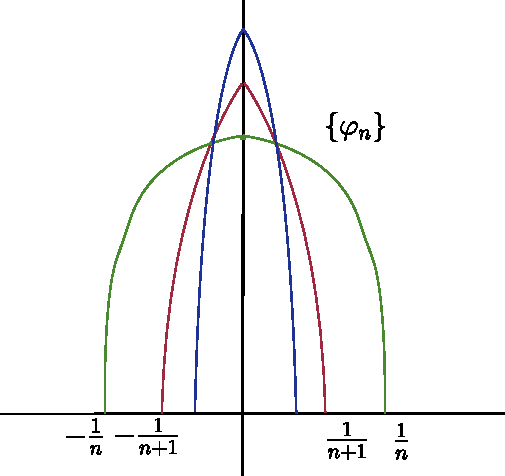
\includegraphics{chapter10/phi_n.pdf}\caption{Теорема 10.3}
\end{figure}
        
\end{theoremwobox} % рисунок

\begin{proof}
    \begin{gather*}
        F(g) = \int^1_{-1} g(x) d\mu = [[\text{раз мера сосредоточена в нуле}]] = g(0) \\
        F_n (g) = \int^1_{-1} g(x) \varphi_n(x) dx = \int^{\frac{1}{n}}_{-\frac{1}{n}} g(x) \varphi_n(x) dx = 
        \intertext{теорема о среднем говорит, что существует такая точка $c_n \in \left[ -\frac{1}{n}, \frac{1}{n} \right]$}
         = g(c_n) \int^{\frac{1}{n}}_{-\frac{1}{n}} \varphi_n(x) dx = g(c_n) \\
        g \in C[-1,1] \Rightarrow \liml_{n \to \infty} g(c_n) = g(0) \Rightarrow \\
        \liml_{n \to \infty} F_n(g) = F(g) \: \forall g \in C[-1, 1] \Rightarrow F = \wstarlim F_n
    \end{gather*}
\end{proof}


\begin{theorem}[Банах-Алаоглу, слабая со * компактность единичного шара сопряженного пространства]
    $X$ --- сепарабельное, нормированное, 
    $D = \seq{f \in X^*, \norm{f} \leq 1}, \: \forall \seq{f_n}^\infty_{n=1}, f_n \in D \: \exists \seq{f_{n_j}}$ --- подпоследовательность 
    $f_0 \in D, f_0 = \wstarlim f_{n_j}$
\end{theorem}

Теорема утверждает гораздо большее на самом деле и могла бы быть даже четвёртвым китом, но четырёх китов не бывает: слишком уж неустойчивая конструкция.


\begin{proof}
    Идея такая: выбрать подпоследовательность из $f_n$, которая будет сходиться на каждом элементе всюду плотного множества в $X$. 
    Выбирать мы будем, используя диагональный процесс.
    \begin{gather*}
        \seq{x_n}^\infty_{n=1} \text{ --- плотное множество в } X \\
        \seq{f_n(x_1)}^\infty_{n=1}, \abs{f_n(x_1)} \leq \norm{f_n} \cdot \norm {x_1} = \norm{x_1} \\ 
        \Rightarrow \seq{f_n(x_1)}^\infty_{n=1} \text{ --- ограниченная последовательность в } \bC 
        \intertext{а из анализа известно, что из ограниченной последовательности можно выбрать сходящуюся подпоследовательность} 
        \Rightarrow \exists \text{ подпоследовательность } \seq{f_{1,n}}^\infty_{n=1} : \: \exists \liml_{n \to \infty} f_{1,n}(x_1) = z_1 \\
        \seq{f_{1,n}(x_2)}^\infty_{n=1}, \abs{f_{1,n}(x_2)} \leq \norm{x_2} \Rightarrow \: \exists \liml_{n \to \infty} f_{2,n}(x_2) = z_2
        \intertext{отметим, что первое условие мы не потеряли, потому что $f_{2,n}$ --- подпоследовательность $f_{1,n}$ и $\liml_{n \to \infty} f_{2,m} (x_1) = z_1$. И так далее, формально говоря, по индукции}
        \seq{f_{j,n}}^\infty_{n=1} \: \liml_{n \to \infty} f_{j,n} (x_k) = z_k, k = 1, 2, \ldots, j \\
        \Rightarrow \liml_{n \to \infty} f_{n,n} (x_j) = z_j \: \forall j \in \bN
    \end{gather*}
    \[ \begin{matrix}
        \textcolor{red}{f_{11}} & f_{12} & f_{13} & \ldots & f_{1n} & \ldots \\
        f_{21} & \textcolor{red}{f_{22}} & f_{23} & \ldots & f_{2n} & \ldots \\
        f_{31} & f_{32} & \textcolor{red}{f_{33}} & \ldots & f_{3n} & \ldots \\
        \vdots &\vdots & \vdots & \vdots & \vdots & \vdots \\
        f_{n1} &\ldots & \ldots & \ldots & \textcolor{red}{f_{nn}} & \ldots \\
        \vdots &\vdots & \vdots & \vdots & \vdots & \vdots \\

    \end{matrix} \]
    Первая строка имеет предел в точке $x_1$, вторая --- подстрочка первой, есть пределы в точках $x_1, x_2$. Каждая  строчка добавляет новый предел. 
    Диагональная последовательность, начиная с некоторого момента ($n \geq j$) на диагонали, будет подпоследовательностью $\seq{f_{j,m}}^\infty_{m=1}$. 
    По замечанию \hyperref[chap10:wstarlim-remark]{10.6} к критерию $\wstarlim$ сходимости $\exists f \in D : f = \wstarlim f_{n,n}$
\end{proof}


\section{Сопряжённые операторы в нормированном пространстве}

\begin{definition}
    $(X, \norm{\cdot}), (Y, \norm{\cdot}), T \in \B(X,Y)$. Определим $T^* : Y^* \rightarrow X^*$: $f \in Y^*, x \in X, (T^* f)(x) \coloneqq f(Tx)$
\end{definition}

\begin{figure}
    \centering
    \begin{tikzpicture}[baseline= (a).base]
        \node[scale=1.2] (a) at (0,0){
            \begin{tikzcd}[every arrow/.append style={shift left}, column sep = huge]
                X \arrow[rr, "T"] \arrow[dr, dashed, "T^*f"] & &Y \arrow[dl, "f"]\\
                & \bC &
            \end{tikzcd}
        };
    \end{tikzpicture}\caption{Определение 10.5, коммутативная диаграмма}
\end{figure}


\begin{theorem}[простейшие свойства сопряженного оператора]
    $(X, \norm{\cdot}), (Y, \norm{\cdot}), T \in \B(X,Y) \Rightarrow$
    \begin{enumerate}
        \item $T^* \in \B(Y^*, X^*), \norm{T^*} = \norm{T}$
        \item $\alpha \in \bC, (\alpha T)^* = \alpha T^*$
        \item $T, S \in \B(X,Y) \Rightarrow (T+S)^* = T^* + S^*$
        \item $(X, \norm{\cdot}), (Y, \norm{\cdot}), (Z, \norm{\cdot}), X \stackrel{T}{\longrightarrow} Y \stackrel{S}{\longrightarrow} Z, T \in \B(X,Y), S \in \B(Y,Z) \Rightarrow 
        (ST)^* = T^* S^* $
    \end{enumerate}
\end{theorem}

\begin{proof}[1]
    Проверим, что $T^* \in \Lin(Y^*, X^*)$
    \begin{gather*}
        \alpha \in \bC, f \in Y^*, x \in X, (T^*(\alpha f))(x) = (\alpha f) (Tx) = \alpha f(Tx) = \alpha(T^*(f))(x) \: \forall x \in X \\
        \Rightarrow T^*(\alpha f) = \alpha T^* (f) \\
        f, g \in Y^*, x \in X, (T^*(f+g))(x) = (f+g)(Tx) = f(Tx) + g(Tx) = \\ =
        (T^*(f))(x) + (T^*(g))(x) \: \forall x \in X
        \intertext{линейность проверили. Теперь посчитаем норму $T^*$}
        \norm{T^*} = \sup_{\{f \in Y^*, \norm{f} \leq 1\}} \norm{T^* f} =
        \intertext{но при фиксированном $f$ у нас получается линейный функционал, поэтому} 
        = \sup_{\seq{\norm{f}_{Y^*} \leq 1}} \left(\sup_{\seq{\norm{x} \leq 1}} \abs{(T^*f)(x)} \right) =
        \intertext{нам ничего не стоит поменять $\sup$ местами. По следствию из теоремы Хана-Банаха для нормированного пространства получаем}
        = \sup_{\seq{\norm{x} \leq 1}} (\sup_{\seq{\norm{f} \leq 1}} \abs{f(Tx)}) = \sup_{\seq{\norm{x} \leq 1}} \norm{Tx} = \norm{T}
    \end{gather*}
\end{proof}

\begin{proof}[2]
    \begin{gather*}
        \alpha \in \bC, f \in Y^*, x \in X \\
        (\alpha T^*)(f)(x) = f((\alpha T)(x)) = \alpha f(Tx) = \alpha(T^*f)(x) \: \forall x, \forall f \Rightarrow (\alpha T)^* = \alpha T^*
    \end{gather*}
\end{proof}

3 доказывается аналогично

\begin{proof}[4]
    \begin{gather*}
        (ST)^*: Z^* \rightarrow X^*, f \in Z^*, x \in X \\
        (((ST)^*)(f))(x) = f((ST)(x)) = f(S(Tx)) = (S^*f)(Tx) = (T^*(S^*f))(x) \\
        \forall x \in X, \forall f \in Z^* \Rightarrow (ST)^* = T^* S^*
    \end{gather*}
\end{proof}

Посмотрим, как выглядит сопряжённый оператор для интегрального оператора. Будем думать, что речь идёт о мере Лебега, чтобы не пугаться каких-то абстрактных мер, хотя Лебег тут совершенно ни при чём.
\begin{theoremwobox}
    \begin{gather*}
        x \in \bR^n, y \in \bR^m, K(x,y)  \in L^p(\bR^{n+m}), 1 < p < + \infty \\
        M = \norm{K}_{L^p} = \left(\int_{\bR^n} \int_{\bR^m} \abs{K(x,y)}^p dx dy\right)^{\frac{1}{p}} \\
        (\K (f))(x) = \int_{\bR^m} K(x,y) f(y) dy, f \in L^q(\bR^m)
    \end{gather*}
    $dx$ в $\bR^n$, $dy$ в $\bR^m$, $dx dy$ --- в $\bR^{n+m}$. Тогда 
    \begin{enumerate}
        \item $\K \in \B(L^q(\bR^m), L^p(\bR^n))$
        \item $(\K^* g)(y) = \int_{\bR^n} K(x,y) g(x) dx $
    \end{enumerate}
\end{theoremwobox}
Ядро сопряженного оператора мы должны записать таким образом, чтобы интегрирование происходило по второй перменной.
    Если мы запишем 2 как $(\K^*g)(y) = \int_{\bR^n} K^*(y,x)g(x)dx$. Сопоставляя эти 2 равенства, мы заключаем, что $K^*(y,x) = K(x,y)$. То есть ядро
    сопряжённого оператора получается перестановкой координат $x$ и $y$.

\begin{proof}[1]
    Справедлива теорема Фубини
    \begin{gather*}
        \int_{\bR^m} \left( \int_{\bR^n} \abs{K(x,y)}^p dx \right) dy < +\infty \Rightarrow \\
        \int_{\bR^n} \abs{K(x,y)}^p dx < +\infty \text{ для п.в. } y \text{ по мере Лебега } dy \text{ в } \bR^m \\ 
        x \in \bR^n \text{ фиксируем}, f \in L^q \\
        \abs{(\K f)(x)} = \abs{ \int_{\bR^m} K(x,y) f(y)dy} \leq [[\text{Гёльдер}]] \left( \int_{\bR^m} \abs{K(x,y)}^pdy \right)^{\frac{1}{p}} \cdot \norm{f}_q
        \intertext{последний интеграл конечен для п.в. $x$. Теперь хотим оценить норму этой штуки в $L^p$} 
        \left( \int_{\bR^n} \abs{\K f(x)}^p dx \right)^{\frac{1}{p}} \leq \norm{f}_q \underbrace{\left(\int_{\bR^n} \left( \int_{\bR^m} \abs{K(x,y)}^p dy \right)dx\right)^{\frac{1}{p}}}_{M} = M \norm{f}_q \\ %attention
        \Rightarrow \K \in \B(L^q(\bR^n), L^p(\bR^n)), \norm{K} \leq M
    \end{gather*}
\end{proof}

\begin{proof}[2]
    \begin{gather*}
        K^*, (L^p(\bR^n))^* = L^q(\bR^n), (L^q(\bR^m))^* = L^p(\bR^m) \\
        \Rightarrow \K^* \in \B(L^q(\bR^n), L^p(\bR^m)) \\
        T \in \B(X,Y), T^* \in \B(Y^*, X^*) \\
        f \in Y^*, x \in X \quad \langle f,Tx\rangle = \langle T^*f, x\rangle \Leftrightarrow (T^*f)(x) = f(Tx)
    \end{gather*}
    $f \in L^p, g \in L^q, \langle f,g\rangle = \int_X fg d\mu, f \in (L^q)^*, f$ действует на $g$ или $g \in (L^p)^*, g$ действует на $f$
    \begin{gather*}
        \langle g, \K f \rangle = \langle \K^*g, f\rangle \quad f \in L^q(\bR^m), g \in L^q(\bR^n) \\
        \langle g, \K f\rangle = \int_{\bR^n} g(x) \left( \int_{\bR^m} K(x,y) f(y) dy \right) dx = 
        \intertext{по теореме Фубини можем переписать}
        = \int_{\bR^m} f(y) \left( \int_{\bR^n} K(x,y) g(x) dx \right) dy \\
        \Rightarrow (\K^*g)(y) = \int_{\bR^n} K(x,y) g(x) dx, g \in L^q(\bR^n) \\
        K^* \text{ --- ядро оператора } \K^* \\
        (\K^* g)(y) = \int_{\bR^n} K^*(y,x) g(x) dx \Rightarrow K^*(y,x) = K(x,y)
    \end{gather*}
\end{proof}

\section{Сопряжённый оператор в гильбертовом пространстве}

\begin{definition}[$T^*$]
    $H$ --- гильбертово, $T \in \B(H), y \in H, y$ --- фиксирован, $x \in H$
    \[ G_y(x) \coloneqq (Tx,y) \]
   из определения $G_y$, очевидно, $G_y \in \Lin(H, \bC)$
    \begin{gather*}
        \abs{G_y(x)} \leq \norm{Tx} \cdot \norm{y} \leq \norm{T} \cdot \norm{x} \cdot \norm{y} \forall x \in H \Rightarrow \\
        G_y \in H^*, \norm{G_y} \leq \norm{T} \cdot \norm{y}
        \intertext{воспользуемся теоремой Рисса \hyperref[chap6:riss]{(тык)}. У нас есть непрервный оператор, значит, есть какой-то элемент, который его порождает}
        \Rightarrow \exists! z \in H \\
        G_y(x) = (x,z)  \: \forall x \in H, \norm{G_y} = \norm{z}
        \intertext{можно было бы написать сразу это, всё выше просто оправдание корректности}
        T^* y \coloneqq z, \text{ то есть } (Tx, y) = (x, T^*y) \: \forall x, y \in H
    \end{gather*}
\end{definition}

$\norm{T^* y} = \norm{G_y} \leq \norm{T} \cdot \norm{y}, T^*$ --- эрмитово сопряжение к $T$. Но слово <<эрмитовость>> скоро отомрёт.

\begin{theoremwobox}[простейшие свойства эрмитово сопряженного оператора]
    .
    \begin{enumerate}
        \item $T^{**} = T$
        \item $T^* \in \B(H), \norm{T^*} = \norm{T}$
        \item $\alpha \in \bC \: (\alpha T)^* = \overline{\alpha} T^*$
        \item $(S+T)^* = S^* + T^*$
        \item $(ST)^* = T^* S^*$
        \item $\exists T^{-1} \Leftrightarrow \: \exists (T^*)^{-1}$ и при этом $(T^*)^{-1} = (T^{-1})^*$
    \end{enumerate}
\end{theoremwobox}

\begin{proof}[1]
    \begin{multline*}
        (Tx,y) = (x, T^*y) = \overline{(T^*y, x)} = \overline{(y, T^{**}x)} = (T^{**}x, y) \: \forall y \in H \\ 
        \Rightarrow Tx = T^{**}x \: \forall x \in H
    \end{multline*}
\end{proof}

\begin{proof}[2]
    $T^* \in \Lin(H)$ --- очевидно. При определении $T^*$ доказали $\norm{T^*y} \leq \norm{T} \cdot \norm{y} \Rightarrow 
    T^* \in \B(H), \norm{T^*} \leq \norm{T}$. Теперь вот такой трюк мы будем часто использовать
      \[  \Rightarrow \norm{T^{**}} \leq \norm {T^*}, \text{ но } T^{**} = T \Rightarrow \norm{T} = \norm{T^*} \]
\end{proof}

\begin{proof}[3]
    \begin{multline*}
        (Tx,y) = (x, T^*y) \Rightarrow ((\alpha T)x, y) = \begin{cases}
             =(x, \overline{\alpha} T^* y) \\ 
             =(x, (\alpha T)^* y)
        \end{cases}
        \Rightarrow (\alpha T)^* = \overline{\alpha} T^*
    \end{multline*}
\end{proof}

4, 5 --- очевидно.

\begin{proof}[6]
    \begin{gather*}
        \text{пусть } \exists T^{-1} \Rightarrow TT^{-1} = I, T^{-1}T = I, I^* = I \stackrel{5}{\Rightarrow} \\
        (T^{-1})^* T^* = I,  T^* (T^{-1})^* = I \\ \begin{cases}
        T^* (T^{-1})^* = I \Rightarrow \: \exists (T^*)^{-1} = (T^{-1})^* \\
        \text{пусть } \exists (T^*)^{-1} \Rightarrow \: \exists (T^{**})^{-1}, \text{ но } T^{**} = T
        \end{cases}
    \end{gather*}
    
\end{proof}

\begin{remark}
    \label{chap10:remark}
    Если $X, Y$ --- банаховы, $T \in \B(X,Y)$
    \[ \exists T^{-1} \in \B(Y,X) \Leftrightarrow \. \exists (T^*)^{-1} \in \B(X^*, Y^*) \]
    и при этом $(T^*)^{-1} = (T^{-1})^*$
\end{remark}

В одну сторону как для гильбертовых пространств, в другую сторону, чтобы доказать похожее, мы пользовались фактом $T^{**} = T$, здесь же 
этого нет. Оставим без доказательства.

\begin{corollary}[интегральный оператор в $L^2$ и его сопряженный]
    \begin{gather*}
        H = L^2(\bR^n, dx), dx = \lambda_n \text{ --- мера Лебега} \\
        K(x,y) \in L^2(\bR^{2n}, d\lambda_{2n}) \quad \left( \int_{\bR^n} \int_{\bR^n} \abs{K(x,y)}^2 dxdy \right)^{\frac{1}{2}} = M < +\infty \\
        (\K f)(x) = \int_{\bR^n} K(x,y) f(y) dy \Rightarrow
    \end{gather*}
    \begin{enumerate}
        \item $\K \in \B(L^2(\bR^n))$
        \item $\K^*$ --- эрмитово-сопряженный 
         \[(K^*g)(y) = \int_{\bR^n} \overline{K(x,y)} g(x) dx, \K^* \in \B(L^2(\bR^n))\]
         \[ (\K^* g)(y) = \int_{\bR^n} K^*(y,x) g(x) dx \Rightarrow K^*(y,x) = \overline{K(x,y)} \] 
    \end{enumerate}
\end{corollary}

Первое утверждение уже доказывали. %мб ссылку
\begin{proof}[2 утверждение]
    \begin{gather*}
        (\K f, g) = (f, K^* g) \quad f,g \in L^2(\bR^n) \\
        (f,g) = \int_{\bR^n} f(x) \overline{g(x)} dx
    \end{gather*}

    \begin{multline*}
        (\K f, g) = \int_{\bR^n} \left( \int_{\bR^n} K(x,y) f(y) dy \right) \overline{g(x)} dx = [[\text{ теорема Фубини }]] \\
        = \int_{\bR^n} f(y) \left( \int_{\bR^n} K(x,y) \overline{g(x)} dx \right) dy = \left(f, \int_{\bR^n}  \overline{K(x,y)} g(x) dx \right) \Rightarrow \\
        \Rightarrow (\K^* g)(y) = \int_{\bR^n} \overline{K(x,y)} g(x) dx
    \end{multline*}
\end{proof}

Введём ещё одно полезное понятие.
\begin{definition}
    $X$ --- нормированное, $T \in \B(X)$. $Y \subset X, Y$ --- подпространство в алгебраическом смысле. $Y$ --- инвариантное подпространство для $T$, если $T(Y) \subset Y$.
\end{definition}
Иными словами, можно рассмотреть сужение оператора на $Y$, это тоже будет оператор.

Прежде чем доказывать что-то простое, сначала небольшое замечание.
\begin{remark}[Проблема Банаха]
    $X$ --- банахово, $T \in \B(X)$. Существует ли замкнутое инвариантное подпространство $(Y \ne \{ 0 \}, Y \ne X)$
\end{remark}

Опять Енфло в 1974 предъявил контр-пример.

Если $H$ --- гильбертово, то ответ неизвестен. Может так, может и не так, никто не знает. Стараются математики, бьются головой, всё бестолку. А мы докажем что-то совсем простое.

\begin{theorem}
    $H$ --- гильбертово, $T \in \B(H)$, $Y$ --- инвариантное подпространство для $T$ $\Rightarrow Y^\perp$ --- инвариантное для $T^*$
\end{theorem}

\begin{proof}
    Просто по определению. Возьмём $x \in Y^\perp, y \in Y$
    \begin{gather*}
        (T^*x, y) = (x, Ty) = 0 \text{ так как } x \in Y^\perp, Ty \in Y \\
        \Rightarrow T^* x \in Y^\perp \Rightarrow T^*(Y^\perp) \subset Y^\perp
    \end{gather*}
\end{proof}

\begin{definition}[самосопряжённый оператор]
    $H$ --- гильбертово пространство. $T \in \B(H), T$ --- \textbf{самосопряжённый}, если $T = T^*$
\end{definition} 
\[ \Leftrightarrow (Tx, y) = (x, Ty) \: \forall x, y \in H \]

\begin{example}
    $H$ --- гильбертово, $M$ --- замкнутое подпространство. $P: H \rightarrow M, P \text{ --- ортогональный проектор, тогда } P = P^*$
\end{example}

\begin{corollary}[из последней теоремы]
    $H$ --- гильбертово, $T \in \B(H), T = T^*$, $Y$ --- инвариантное подпространство для $T \Rightarrow Y^\perp$  ---
    инвариантное подпространство для $T$
\end{corollary}

\begin{theorem}[о ядре и образе оператора и его сопряженного]
    $H$ --- гильбертово пространство, $T \in \B(H) \Rightarrow$
    \begin{enumerate}
        \item $H = \Ker T \oplus \overline{T^*(H)}$ ($\overline{T^*(H)}$ --- замыкание образа)
        \item $H = \Ker T^* \oplus \overline{T(H)}$ 
    \end{enumerate}
\end{theorem}
 
Такое часто бывает полезно при разложении гильбертова пространства.

\begin{proof}
    Сначала сделаем абстрактное замечание. Пусть $L$ --- подпространство в алгебраическом смысле для $H$ (не обязательно замкнутое, даже интереснее, если оно не замкнутое). 
    Может, мы когда-то уже отмечали, что $L^\perp = \overline{L}^\perp$. Если $M = \{x : x \perp L  \} = \{x : x \perp \overline{L}\} \Rightarrow$ 
    \begin{gather*}
        H = \overline{L} \oplus M \\
        \text{в нашем случае будет }L \coloneqq T^*(H)\\
         \text{вычислим } L^\perp \\
        \text{пусть } x \perp T^*(H) \Leftrightarrow 0 = (x, T^*y) \: \forall y \in H \Leftrightarrow \\
        \Leftrightarrow 0 = (Tx, y) \: \forall y \in H \Leftrightarrow Tx = 0 \Leftrightarrow x \in \Ker T \\
        \Rightarrow H = \Ker T \oplus \overline{T^*(H)}
        \intertext{применим 1 к $T^*$}
        \Rightarrow H = \Ker T^* \oplus \overline{T^{**}(H)}, T^{**} = T
    \end{gather*}
\end{proof}

\end{document}
